\section{\inGerman{Funktionsweise von RetroShare}\inEnglish{How RetroShare works}}
\inGerman{In diesem Kapitel sollen alle verschiedenen Möglichkeiten der Kommunikation in RetroShare aufgelistet werden und erklärt werden.
Dazu soll dieses fiktive RetroShare Netzwerk betrachtet werden mit 8 Teilnehmern. Ein Strich zwischen zwei Teilnehmern soll bedeuten, dass sich beide gegenseitig als Freunde hinzugefügt haben. Zur Vereinfachung sei nun auch angenommen, dass alle Teilnehmer zur Zeit online sind.}
\inEnglish{This chapter should list and explain the various ways of communication in RetroShare and how they are working.
We will assume the following fictive RetroShare-Network with 8 participants. A line between two nodes should indicate that those two users are friends with each other. For simplification purposes, we assume that all 8 users are online, too.}

\begin{center}
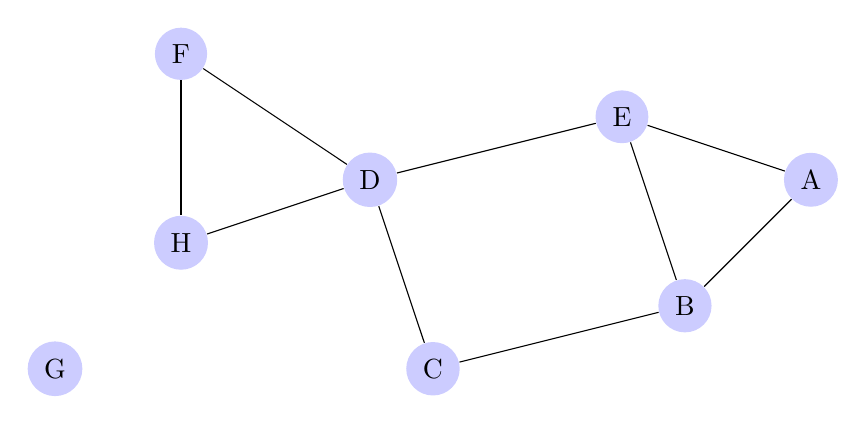
\begin{tikzpicture}
  [scale=.8,auto=left,every node/.style={circle,fill=blue!20}]
  \node (n6) at (1,10) {F};
  \node (n4) at (4,8)  {D};
  \node (n5) at (8,9)  {E};
  \node (n1) at (11,8) {A};
  \node (n2) at (9,6)  {B};
  \node (n3) at (5,5)  {C};
  \node (n7) at (-1,5)  {G};
  \node (n8) at (1,7)  {H};
  \foreach \from/\to in {n6/n4,n4/n5,n5/n1,n1/n2,n2/n5,n2/n3,n3/n4,n8/n4,n8/n6}
    \draw (\from) -- (\to);
\end{tikzpicture}
\end{center}
\inGerman{Person G hat gerade RetroShare installiert und noch keinen Freund. Person E ist mit A, B und D befreundet u.s.w.}
\inEnglish{User G has installed RetroShare just this minute and not yet added friends. User E ist friends with A, B und D and so forth...}

\inGerman{Im folgenden sei ein \underline{Freund} jeweils eine direkt mit dir befreundete Person, ein \underline{Freundesfreund} ein Freund einer deiner Freunde, mit dem du nicht befreundet bist. Wenn du z.B. die Person A wärst, wären deine Freunde E und B, deine Freundesfreunde C und D, und F bzw. H wären dann \underline{Freunde dritter Stufe}.}
\inEnglish{We shall call below ``a friend'' a person, which you have added as friend. A ``friend second grade'' shall be a friend of a friend of yours, with whom you are not friends. If f.e. you are person A, your friends would be E,B, your friends second grade would be C and D and the users F and H would be friends third grade to you.}

\inGerman{\emph{RetroShare verbindet sich ausschließlich mit direkten Freunden}, nicht mit Freundesfreunden.
Daher ist die Nutzung von RetroShare zu 100\% sicher, wenn man seinen Freunden vertrauen kann.
Eine kleine Ausnahme davon ist - falls eingeschaltet - das DHT, dazu im nächsten Abschnitt mehr.}
\inEnglish{\emph{RetroShare connects ONLY to your direct friends}, but not to your friends second or higher grade. So if you're adding only thrustworthy persons, you can be 100\% safe. The only (and small) exception to this rule is the DHT, see below for details.}

\inGerman{Person G kann RetroShare nicht benutzen, da er keine Freunde hat.
Würde nun D offline gehen, so würde sich dieses Netzwerk in zwei Unternetzwerke aufteilen, und somit wäre z.B. ein Dateitransfer zwischen H und A unmöglich.}
\inEnglish{So, a basic consequence is that G can't use RetroShare, because he has no friends.
If user D goes offline, the above RetroShare-network will split in two subnetworks and no communication or file transfer is possible between H and A anymore.}

\subsection{\inGerman{Verbindung zu Freunden}
\inEnglish{Connection with friends}} \label{ip_determination}
\inGerman{Die meisten Personen haben privat daheim keine statische IP Adresse, sondern eine sogenannte dynamische, die sich regelmäßig (meist alle 24h) ändert.
Das Problem dabei ist, dass RetroShare auch in der Lage sein muss, sich zu verbinden, wenn du und dein Freund beide für länger als 24h offline wart.
Dazu verwendet RetroShare je nach Einstellung bis zu drei verschiedene Methoden, die in den folgenden Unterkapiteln erklärt werden sollen.}
\inEnglish{Most people don't have a static ip address at home, instead they have a so called dynamic IP, which changes every 24 hours.
This is a problem, as RetroShare should be able to connect to your friend, if you and your friend are offline for more than 24 hours.
To get the IP address of your friend, RetroShare uses three different methods, which should be explained in the following subsections.}

\inGerman{Ich persönlich habe immer DHT und Discovery an, beides auszuschalten ist nur nötig, wenn die Benutzung von RetroShare selbst illegal wäre, wie vermutlich z.B. in China.}
\inEnglish{Personally, I've always DHT and Discovery activated, because deactivating both will make connections more complicated and I don't need to hide I'm using RetroShare, because I live in a free country.}

\subsubsection{DHT} \label{dht}
\inGerman{Das ``Distributed Hash Table'' ist die einfachste und bequemste Methode.
Dabei nutzt RetroShare momentan noch das ``Bittorrent-DHT'', das wohl größte weltweit.
Beachte, dass sich RetroShare hier ausnahmsweise auch mit dritten verbindet, allerdings nur um die IP-Adressen deiner Freunde nachzuschlagen.}
\inEnglish{The ``Distributed Hash Table'' is the easiest and comfortablest method.
RetroShare uses the ``Bittorrent-DHT'', the probably biggest world wide.
You should know, that RetroShare will make connections to strangers here, but ONLY to look up the IP-adresses of your friends.}

\inGerman{RetroShare wird dort in diesem verteilten Netzwerk einen Eintrag der Form (SSL-ID, IP-Adresse)  erzeugen.
Damit kann dann jeder, der deine SSL-ID kennt (deine Freunde und wenn du Discovery aktiviert hast, deine Freundesfreunde), deine IP Adresse bestimmen.
Wer deine SSL-ID nicht kennt, weiß nur, dass hinter deiner IP-Adresse ein RetroShare Nutzer steckt, mehr aber auch nicht, insbesondere nicht deinen RetroShare-Namen.}
\inEnglish{RetroShare will create an entry in this distributed network, which has the format (your SSLID, IP-adress).
Everyone, who knows your SSL-ID (your friends and - if you have Discovery turned on - your friends of friends), can determine your IP-Adress then.
People, who don't know your IP-adress, can only determine, that someone behind this IP is using RetroShare, but not the RetroShare nick, which friends he has or what he does.}

\inGerman{Wer das DHT nicht aktiviert, dem sei dringend die Einrichtung einer dynamischen DNS empfohlen, siehe weiter unten.}
\inEnglish{If you don't want to make public, that your IP is using RetroShare, and you want to turn it off, you should setup Dynamic DNS, see section \ref{dyndns}.}

\inGerman{Das DHT stellt mit vielen Personen gleichzeitig eine Verbindung her, was manche Router nicht vertragen zu scheinen.
Dies äußert sich in ständigen Verbindungsabbrüchen zu deinen Freunden.}
\inEnglish{The DHT makes a bunch of connections at the same time, and some consumer routers don't like that.
This results in connection losses every five minutes or so.}

\subsubsection{Discovery} \label{discovery}
\inGerman{Bei Discovery erlaubst du deinen Freunden, deinen Schl\"ussel und deine IP an deren Freunde weiterzugeben, d.h. an deine Freunde zweiter Stufe.
Zudem teilst du allen deinen Freunden mit, mit wem du befreundet bist.
Dies hat zwei Folgen:}
\inEnglish{With Discovery turned on, you allow your friends, to give your key and your IP to all of their friends, i.e. to your friends of second grade.
Moreover, you send your friendlist to all of your friends.
This implies two things:}
\begin{itemize}
\item
\inGerman{\emph{Zu dir kann leichter verbunden werden.}
Stell dir vor, du bist im obigen Netzwerk F und du bist mit D verbunden bist, H ist offline.
Nun kommt H online, weiss aber zun\"achst nur die IP von D und verbindet sich mit diesem.
Wenn du Discovery an hast, wird nun D deine IP an H schicken, und H kann sich zu dir verbinden.}
\inEnglish{\emph{It's easier to connect to you.}
Imagine, you are F in the network above and you're currently connected to D, H is offline.
Now H goes online, but knows only the IP of D and connects to him.
If you have discovery on, D now will send your IP to H and H can connect to you.}
\item
\inGerman{\emph{Es ist einfacher, mit dir Freund zu werden.}
Angenommen, du bist wieder F und du und E m\"ochten nun Freunde werden.
Wenn du Discovery an hast, hat E nun schon deinen Schl\"ussel von deinem Freund D geschickt bekommen, und somit ist das Adden nun nur noch ein Mausklick.
Der umst\"andliche Austausch von Zertifikaten ist nun nicht mehr n\"otig.}
\inEnglish{\emph{It is easier, to become friends with you, if you want to.}
Imagine, you're F again, and you and E want to be friends now.
If you have Discovery turned on, E will already have your key (your common friend D has sent your key) and adding friends is only a mouseclick anymore.
The annoying manual key exchange is no longer necessary.
}
\end{itemize}

\subsubsection{DynDNS} \label{dyndns}
\inGerman{Die wohl beste Methode ist es, dass du selbst eine sogenannte ``dynamische DNS'' einrichtest.
Dazu kannst du z.B. auf der Seite \url{http://no-ip.org} oder diversen anderen eine dynamische DNS der Form ``irgendwas.no-ip.org'' registrieren und diese von deinem PC oder am besten sogar deinem Router direkt aktualisieren lassen, falls sie sich geändert hat.}
\inEnglish{The best method to increase your connectivity is the setup of ``dynamic DNS''.
You need to go to a site like \url{http://no-ip.org} and register a dyndns like ``something.no-ip.org''.
This DNS entry can be updated from your PC regularly or (even better) directly by your router.}

\inGerman{Das Einrichten einer dynamischen DNS soll hier nicht weiter erklärt werden, da es den Rahmen sprengt.}
\inEnglish{The setup of dynamic DNS is beyond the scope of this document, just google it.}

\inGerman{Deine Freunde bzw. deren RetroShare kann dann einfach die DNS ``irgendwas.no-ip.org'' nachschlagen und kann deine IP-Adresse sofort ermitteln.}
\inEnglish{Your friends (resp. their RetroShare) can then make a simple DNS query and will get your current IP.}

\inGerman{Mit einer funktionierenden DynDNS Einrichtung kann DHT und Discovery ausgeschaltet werden.}
\inEnglish{With a working DynDNS setup, you can disable DHT and Discovery.}

\subsection{Chat}
\inGerman{RetroShare unterstützt Instant-Messaging mit direkten Freunden. Einfach in der Freundesliste auf den Namen doppelt klicken und das Chatfenster öffnet sich.}
\inEnglish{RetroShare allows Instant Messaging with your direct friends. Just doubleclick in the friends list on a name and the chat window opens.}
 
\inGerman{Nachrichten, die du deinem Freund schreibst, während er offline ist, werden erst zugestellt, wenn du und dein Freund wieder miteinander verbunden sind! Sie werden ja nicht wie üblich auf einem Server zwischengespeichert.}
\inEnglish{Beware: Messages, which your writing when your friend is offline, will be not be delivered until you and your friend are connected again! There is no central server, which could save the messages for you, as you might be used to. }

\subsection{\inGerman{Gruppenchat}\inEnglish{Group Chat}}
\inGerman{Im Gruppenchat können Nachrichten an alle Freunde, die online sind gesendet werden. Freunde, die gerade offline sind, erhalten diese nicht.}
\inEnglish{Using the group chat allows you to send a message to all of your direct friends which are online. Offline friends won't get the message, even if they get online later.}

\inGerman{Das f\"uhrt dazu, dass man im Gruppenchat nur ``Gespenst''-Chats mitlesen kann, d.h. nur die Nachrichten von einer Person. Denn unterhalten sich z.B. E und D im Gruppenchat, so kann die komplette Konversation nur von E und D mitgelesen werden, hingegen erhalten A und B nur die Nachrichten von E, und C,F,H können nur die Nachrichten von D lesen.}
\inEnglish{This has the consequence, that you'll notice ``ghost-chats'' in the group chat window sometimes, i.e. you can read only the messages of one person. For example, if E and D are chatting using the group chat, only those two can read both parts of the conversation. A and B will get only the messages from E, and C,F,H will only get D's messages.}

\inGerman{Der Gruppenchat ist meiner Meinung nach nur für Meldungen wie z.B. ``Ich bin die nächsten 4 Tage offline.'' etc. nützlich.}
\inEnglish{The group chat is probably not the most useful feature, I use it only for messages like ``I'm offline the next week.''.}

\subsection{\inGerman{Nachrichten}\inEnglish{Messages}}
\inGerman{Ähnlich wie der Chat funktioniert auch das Versenden von Nachrichten. Diese können nur zugestellt werden, wenn der Empfänger zur selben Zeit wie du online ist.
Falls also A an B eine Nachricht schreibt, aber A immer nur von 8 bis 12 Uhr online ist, B hingegen nur von 13-18 Uhr, so wird diese Nachricht niemals zugestellt werden.}
\inEnglish{The delivery of messages is similar to the delivery of chat messages. They will only be delivered, if you and your friend are connected, otherwise the messages will stay in the outbox. So, if A is writing a message to B, but A is online only from 8am to 12am, B instead only from 1pm to 6pm, the message will never be delivered.}

\subsection{\inGerman{Datei Transfer}\inEnglish{File Transfer}} \label{filetransfer}

\inGerman{Das fortgeschrittenste Feature an RetroShare ist wohl der Austausch von Dateien. Bei der Freigabe von Dateien gibt es drei Möglichkeiten, wie die Dateien freigegeben werden sollen, nämlich
\begin{itemize}
 \item netzwerkweit
 \item durchsuchbar von Freunden
 \item durchsuchbar von ein oder mehreren Gruppen von Freunden
\end{itemize}
Es macht natürlich keinen Sinn, in RetroShare Dateien freizugeben ohne mindestens eine der drei Freigabetypen auszuwählen, da die Dateien sonst gar nicht wirklich freigeben werden.
Was genau die beiden Freigabetypen bedeuten, soll in den beiden folgenden Unterkapiteln behandelt werden.}
\inEnglish{Probably the most advanced feature of RetroShare is the exchange of files. Everyone can share one or more folders, and there are the following three options:
\begin{itemize}
 \item networkwide
 \item browsable by friends
 \item browsable only by a group of friends
\end{itemize}
Of course, it is pointless to adding a folder, without at least one of those options enabled. 
What those options mean, will be explained in the next chapters.}

\subsubsection{\inGerman{durchsuchbare Freigaben}\inEnglish{browsable by friends}}
\inGerman{Diese Art von Freigabe eignet sich am besten für private Dateien, wie z.B. Urlaubsfotos. Alle direkten Freunde von dir sehen diese Dateien in ihrem ``Dateien'' Fenster und können dort das Herunterladen in Auftrag geben.}
\inEnglish{This option allows all your direct friends to see and browse this folder in their ``Files'' Tab. They can download then the complete folder or some parts of it.}

\inGerman{Sobald sie dies tun, wirst du diese Dateien in deinem Upload Fenster sehen und dort auch den Namen des Freundes, der diese herunterlädt. Auch der Freund sieht deinen Namen als Quelle der Datei, die er herunterlädt.}
\inEnglish{As soon as your friend starts downloading some browsable shared files, you'll see his name and the file in the upload window.}

\inGerman{Insbesondere weiß jeder deiner Freunde, dass du diese Datei freigegeben hast.}
\inEnglish{Noteworthy is, that all your friends will know that these files are from you.}

\subsubsection{\inGerman{Anonyme Freigaben}\inEnglish{Anonymous shares}}
\inGerman{Diese Art von Freigabe eignet sich dazu, dass nicht einmal Freunde sicher wissen können, was du freigegeben hast.}
\inEnglish{This option of sharing a folder allows you to share files, without your friends knowing it.}

\inGerman{In diesem Abschnitt seist du Person A aus obigem Graph, und du hast einen Ordner ``Test'' mit der Datei ``Testdatei'' nur anonym, nicht aber durchsuchbar freigegeben. Insbesondere taucht dieser Testordner nicht im Tab Dateien auf und kann nur \"ueber die Suche gefunden werden.}
\inEnglish{In this subsection, we'll assume that you are person A from the above graph, and you are sharing the folder ``Test'', which contains the file ``Testfile''. Nobody will see this folder in his ``Files'' tab then, it can only be found using the search function.}

\inGerman{Angenommen F sucht nun nach dem Begriff ``Testdatei''.
F schickt seine Suchanfrage nach D, D leitet die Suchanfrage weiter an E und C,  usw. und irgendwann landet die Suchanfrage bei dir und du meldest einen Treffer.
Jeder Knoten hat sich nun kurzzeitig gemerkt von wem er an wen die Suchanfrage weitergeleitet hat (z.B. merkt sich E: ``Ich habe die Suchanfrage nach ''Testdatei`` und der ID 128931 von D nach A weitergeleitet.'').
So ist es möglich, dass du deinen Treffer an F zurücksenden kannst, ohne dass irgendein Knoten sichere Information hat, wer gesucht und wer den Treffer hat.}
\inEnglish{Let's assume, that F searches for ``Testfile''.
F sends a search request to D, D forwards this request to E and C, and so on, and after a few hops, the search request arrives at you and you - having ``Testfile'' - send a hit back.
Every node has a temporary cache, from who he forwarded which search request to whom (e.g. E remembers: I have forwarded the search request for ``Testfile'' with the ID 128931 from D to A).
This way, it is possible, that your success message can be sent the same way back to F, without any node between knowing who searched and who had the hit.}

\inGerman{So können ``Anonyme F2F Tunnel'' über maximal 6 Knoten aufgebaut werden und man kann auch Dateien netzwerkweit tauschen, ohne jemals Dateien an andere außer deinen Freunden zu senden.}
\inEnglish{This way, it is possible to establish ``Anonymous F2F tunnels'' up to a maximum of 6 hops and you can share files networkwide, without ever making a connection with other peers except your friends.}

\inGerman{Betrachten wir nun, was jeder Teilnehmer eines solchen ``Anonymer F2F-Tunnel'' weiß, am Beispiel des obigen Tunnels A $\leftrightarrow$ E $\leftrightarrow$ D  $\leftrightarrow$ F:
\begin{itemize}
 \item A weiß, dass er die Datei ``Testdatei'' an seinen Freund E hochlädt. (In der GUI wird im Upload Fenster nur ``Anonymer F2F-Tunnel'' angezeigt). Er weiß nicht, ob E diese Datei angefordert hat, oder E sie nur weiterleitet.
 \item E weiß nur, dass er eine Datei von A nach D weiterleitet. Er kann den Inhalt der Datei einsehen, weiß aber nicht, ob A sie hochlädt, oder E sie herunterlädt.
 \item Analog weiß D nur, dass er eine Datei von E nach F weiterleitet, könnte jedoch den Inhalt des weitergeleiteten anschauen.
 \item F weiß nur, dass er die Datei ``Testdatei'' von D herunterlädt. Er weiß nicht, ob D sie hochlädt oder nur weiterleitet.
\end{itemize}}
\inEnglish{Let's look at the information, each participant of this ``Anonymous F2F-Tunnel'' knows, looking at the example tunnel A $\leftrightarrow$ E $\leftrightarrow$ D  $\leftrightarrow$ F from above.
\begin{itemize}
\item A knows, that he is uploading the file ``Testfile'' to his friend E. (In the GUI, he'll see as Peer only ``Anonymous F2F-Tunnel''). He doesn't know, if E requests this file, or E forwards this file.
\item E knows, that he forwards a file from A to D. He could spy on what he is transferring, but he can't say, if A is uploading the file or E is downloading it. They could both forward this file from someone else.
\item Analogue, D knows, he's forwarding a file from E to F and he could look at the file.
\item F knows, that he is downloading the file ``Testfile'' from D, but he doesn't know, if D shares this file, or is just forwarding it.
\end{itemize}}

\inGerman{Natürlich wird die Downloadgeschwindigkeit bei längeren Tunneln meist recht langsam sein, hängt sie doch vom ``schwächsten'' Glied der Kette ab. 
Hat z.B. E nur einen sehr langsamen Internetanschluss, so wird die Verbindung zwischen F und A auch sehr langsam sein.}
\inEnglish{Of course, the download speed of a long tunnel will most of the time be very slow, because it depends on the weakest link in the chain.
If e.g. E has only a very slow internet connection, tunnels between F and A will be slow, too.}

\inGerman{Die Nachteile an anonymen Freigaben sind, dass diese nur über die Suche gefunden werden können und zudem nicht das Tauschen in Ordnerstrukturen erlauben.
Möchte man nun trotzdem einen kompletten Ordner dem gesamten RetroShare Netzwerk komfortabel zum Download anbieten, so ist die beste Methode, für diesen Ordner eine Kollektion (siehe \ref{rscollection}) zu erstellen und anschließend den RetroShare-Link zu dieser ``.rscollection''-Datei in einem Forum zu posten.}
\inEnglish{The downsides of anonymous shares are, that other people can find those only by using the search and that they don't allow sharing complete folders.
If you want to share a complete folder with the whole network anyway, the best way is, to create a collection (see section \ref{rscollection}) and then post the link to this collection file anonymously in a forum.}
 
\inGerman{Genauere technische Details gibt es in der offiziellen Dokumentation \url{http://retroshare.sourceforge.net/wiki/index.php/Documentation:TurtleHopping}.}
\inEnglish{More about technical details can be read at the official documentation \url{http://retroshare.sourceforge.net/wiki/index.php/Documentation:TurtleHopping}.}

\subsubsection{Swarming}
\inGerman{RetroShare unterstützt das Torrent-Prinzip, d.h. jeder, der eine Datei herunterlädt, kann diese im selben Moment schon wieder hochladen.
Auch der Download von mehreren Quellen gleichzeitig ist möglich.}
\inEnglish{RetroShare is capable of the so called ``swarming'', i.e. everyone, who downloads a file, can upload this at the same moment without having the complete file.
The download from multiple sources is possible, too.}

\inGerman{Jede Datei wird dazu in Blöcke von 1MB geteilt und ausschließlich über den Hash der Datei identifiziert, d.h. haben zwei User dieselbe Datei mit anderem Namen, so kann ein dritter User trotzdem von beiden diese Datei herunterladen.}
\inEnglish{Every file is divided into chunks of 1MB and the file is only identified by the hash, i.e. if two users have the same file with different names, a third user can still download from both of them.}

\subsubsection{RetroShare-Links}

\inGerman{RetroShare-intern können Links zu Dateien verbreitet werden. Ein Beispiel-Link wäre}
\inEnglish{There exists RetroShare-internal links to files. A example link is:}

retroshare://file?{\color{green}name=RSCounterFile.txt}\&{\color{yellow}size=200}\&{\color{red}hash=d89f3b4f3fe842ac9164fb19b8d1ab6b2e238d61}

\inGerman{Man sieht, dass dieser nur aus den folgenden Komponenten besteht:
\begin{itemize}
 \item {\color{green}Dateinamen}: Dieser teilt RetroShare mit, unter welchem Namen es die Datei nach dem Download abspeichern soll. Dieser kann beliebig verändert werden, der Link funktioniert trotzdem noch.
 \item {\color{yellow}Dateigröße}: RetroShare muss die Größe der Datei wissen.
 \item {\color{red}Hash}: Über den Hash identifiziert RetroShare, welche Datei es herunterladen soll. Es ist dabei sehr, sehr unwahrscheinlich, dass zwei Dateien weltweit denselben Hash haben.
\end{itemize}}
\inEnglish{You can see, that such a link consists only of the following components:
\begin{itemize}
\item {\color{green}the file name}: This name is the name, RetroShare saves the file to. It can be modified arbitrarily and the link is still valid.
\item {\color{yellow}file size}: RetroShare needs to know, how big the file is.
\item {\color{red}Hash}: The SHA1 hash of the file is used, to identify which file should be downloaded. It's very very unlikely, that two files worldwide have the same hash.
\end{itemize}}

\subsubsection{\inGerman{RetroShare-Kollektionen}\inEnglish{RetroShare-Collections}} \label{rscollection}

\inGerman{Mittels ``.rscollection''-Dateien können auch komplette Ordner samt Unterordner und allen enthaltenen Dateien bequem heruntergeladen werden.
Eine RSCollection ist dabei nur eine Datei mit der Endung ``.rscollection''.
Es handelt sich dabei um eine XML-Datei, sie enthält eine Ordnerhierarchie und die dazugehörigen Hashs.
Ein Beispiel für den Inhalt einer Collection-Datei wäre:}
\inEnglish{With *.rscollection files, complete folders with subfolders and all contained files can easiliy be downloaded.
A collection is simply a XML file, which contains the folder structure and all names/hashes of the files.
An example collection looks like this:}

\begin{lstlisting}
<!DOCTYPE RsCollection>
<RsCollection>
 <Directory name="Mainfolder">
  <File size="100" sha1="23f744d9b68841f31e4fe24473066a794898a5bc" name="file1.txt"/>
  <File size="100" sha1="5f695778740e9f7f63022083f62a09ecc07aaa35" name="file2.txt"/>
  <Directory name="Subfolder">
   <File size="200" sha1="2cc55a96942996e1cf870ee43bb269a5cd57d342" name="file3.txt"/>
   <File size="200" sha1="e84e958c18b2fa3e2014c347f7e974e2b797523f" name="file4.txt"/>
  </Directory>
 </Directory>
</RsCollection>
\end{lstlisting}
\inGerman{Diese 4 Dateien in dieser RSCollection k\"onnten nun heruntergeladen werden, indem diese Kollektion mittels des Buttons ``\"Offne Kollektion'' im Transfers-Fenster geoeffnet wird. 
Dadurch wird zuerst im eingehenden Ordner zuerst die richtige Ordnerstruktur erstellt (im Beispiel die Ordner ``incoming/Hauptordner'' und ``incoming/Hauptordner/Unterordner'') und anschließend alle ausgewählten Dateien zum Download in Auftrag gegeben.
Nachdem der Download einer Datei abgeschlossen ist, wird diese automatisch in den passenden Unterordner kopiert.}
\inEnglish{These 4 files of this RSCollection can now be downloaded by using the button ``Open Collection'' in the Transfers-tab.
If you do this, RetroShare will create the folder structure for you (in the example the folders ``incoming/Mainfolder'' and ``incoming/Mainfolder/Subfolder'') and then queue all 4 files in the download queue.
After finishing the download of one of those 4 files, it'll be moved into the correct subfolder automatically.}

\subsection{Foren} \label{foren}

\inGerman{Foren erlauben den dezentralen Austausch von Nachrichten mit beliebig weit entfernten Teilnehmern des Netzwerkes. Jeder Teilnehmer kann ein Forum erstellen, dieses Forum sehen dann zunächst alle Freunde des Erstellers.}
\inEnglish{}

\inGerman{Foren verbreiten sich nur weiter, indem jemand sie abonniert. Dies dient dazu, dass Spam verhindert wird. Jeder, der ein Forum abonniert, verbreitet dieses an alle seine Freunde weiter. So gesehen ist das Abonnieren eines Forums auch eine Empfehlung dieses Forums an deine Freunde. Das Schreiben von Artikeln in Foren ist nur möglich, falls man dieses Forum abonniert hat.}
\inEnglish{}

\inGerman{Foren können nur gelöscht werden, indem jede Person das Abonnement kündigt. Solange noch eine Person das Forum abonniert hat, ist dieses auch noch im Netzwerk verfügbar. Du kannst also auch bei selbsterstellten Foren das Abonnement kündigen.}
\inEnglish{}

\inGerman{Im Beispiel funktioniert das so: Erstellt A ein Forum, so können es also A, B, D sehen. Abonniert B noch zusätzlich dieses Forum, so können es nun A, B, C, E sehen. Möchte A nun das Forum löschen, so kann er diesem das Abonnement kündigen, jedoch wird das Forum trotzdem noch für B und dessen Freunde sichtbar bleiben (also A, B, C, E), bis auch B sich austrägt und das Forum endgültig nicht weiter verteilt wird. Bei allen Leuten, die dieses Forum jedoch einmal gesehen haben (hier A,B,C,E), bleiben die Nachrichten momentan im Cache und somit für alle Zeit erhalten.}
\inEnglish{}

\inGerman{In der momentanen Implementation verschwinden Foreneintr\"age nach gut einem Jahr.}
\inEnglish{With the current implementation, RetroShare discards forum messages after some more after a year.}

\subsubsection{\inGerman{AUTHentifizierte Foren}\inEnglish{AUTHenticated Forums}}
\inGerman{Bei authentifizierten Foren wird für jede Nachricht eine gültige Unterschrift verlangt.
Somit ist einsehbar, welcher Person (genauer welcher PGP Schlüssel) diese Nachricht erstellt hat.}
\inEnglish{If a forum is Authenticated, a signature is required for each message.
This ensures, that everybody knows, which person (more precisely which PGP key), created this message.}

\inGerman{Falls die Unterschrift nicht verifiziert werden kann, da der PGP-Schlüssel mit der passenden ID nicht bekannt ist (z.B. Nachricht von jemanden, der weder Freund noch Freundesfreund von dir ist), so wird hier eine ``Fehlende Nachricht'' angezeigt.
Somit sind von dir geschriebene Nachrichten auch maximal von Freundesfreunden lesbar und Nachrichten verbreiten sich nicht beliebig weit im RetroShare-Netzwerk.}
\inEnglish{If the signature can't be verified by your RetroShare, because the PGP-key with the related ID is not known (e.g. a message from someone, which is a friend of third or more grade), this message won't be displayed.
This has the consequence, that you can read only messages from friends or friends of second grade.
You'll get the other messages, too, but the current implementation won't display it.}

\subsubsection{\inGerman{Anonyme Foren}\inEnglish{Anonymous Forums}}
\inGerman{Bei authentifizierten Nachrichten ist keine Unterschrift erforderlich und somit kann jeder anonym schreiben.
Nachrichten verbreiten sich beliebig weit, und niemand weiß, wer eine Nachricht geschrieben hat.}
\inEnglish{In anonymous forums no signature is required and everyone can post anonymously.
Thus, messages distribute infinitely far and can be read by everyone, who can read this forum.}

\inGerman{Optional kann man seine Nachrichten trotzdem unterschreiben, damit den anderen klar wird, dass die Nachricht in dem anonymen Forum auch wirklich von dir stammt. Somit kann auch in anonymen Foren ein Nachweis erbracht werden, wer die Nachricht geschrieben hat.}
\inEnglish{You can - if you want to - still sign the messages, so everyone with your key knows, that the message is from you. This makes it even in anonymous forums possible to prove that a certain message is from a certain person.}

\subsection{\inGerman{Kanäle}\inEnglish{Channels}}
\inGerman{Ein Kanal ermöglicht es einer Person neue Nachrichten bzw. Dateien RetroShare-intern zu veröffentlichen.
Ich sehe in meiner Liste z.B. einen Kanal mit aktuellen Versionen von RetroShare als auch einen Kanal mit IT-News.}
\inEnglish{A channels allows a person to spread new messages or files. I can see e.g. a channel with current RetroShare builds as well as a channel with IT-News.}

\inGerman{Die Sichtbarkeit von Kanälen ist dabei genauso wie die Sichtbarkeit von Foren, für Details siehe dazu das Kapitel \ref{foren}.}
\inEnglish{}

\inGerman{Für jeden Kanal wird ein GnuPG-Schlüssel erzeugt. Jeder der den privaten Schlüssel dieses Kanals besitzt kann dort neue Nachrichten schreiben. Bei der Erstellung kann man auswählen, ob nur man selbst oder einige ausgewählte Personen diesen privaten Schlüssel erhalten und somit veröffentlichen können (Regelfall) oder jede Person (nicht besonders nützlich meiner Meinung nach).}
\inEnglish{}

\inGerman{Das Abonnieren eines Kanals führt dazu, dass dort veröffentliche Dateien automatisch heruntergeladen werden, dies kann jedoch auch deaktiviert werden.}
\inEnglish{}

\subsection{Chatlobbies}
\inGerman{Chatlobbies ermöglichen es auch mit nicht befreundeten Personen dezentral zu chatten. Im Beispiel oben könnten somit F, D, E und A miteinander chatten.}
\inEnglish{}

\inGerman{Bei Chatlobbies findet niemals eine Authentifizierung statt, jeder kann sich mit einem beliebigen Namen in der Chatlobby anmelden!
Seinen Nicknamen kann man in den Optionen im Unterpunkt ``Chat'' ändern.
Insbesondere könnte Person A als Nicknamen auch ``Person B'' wählen und somit sich als jemand anderes ausgeben!}
\inEnglish{}

\inGerman{Es gibt sowohl öffentliche Chatlobbies, die jeder Nutzer sieht, als auch private, die man nur nach Einladung eines Mitglieds sieht.}
\inEnglish{}

\inGerman{Genaue technische Details findet man auf der offiziellen Dokumentationsseite \url{http://retroshare.sourceforge.net/wiki/index.php/Documentation:ChatLobbies}.}
\inEnglish{}

\subsubsection{private Chatlobbies}
\inGerman{Private Chatlobbies sieht man nur, indem man eine Einladung dazu erhält. Leider sind private Chatlobbies zur Zeit etwas benutzerunfreundlich, denn started man RetroShare neu, so muss man von einem Mitglied, dass noch in der privaten Chatlobby ist, wieder neu eingeladen werden.}
\inEnglish{}

\subsubsection{öffentliche Chatlobbies}
\inGerman{Ist mindestens ein Freund von dir in einer öffentlichen Chatlobby eingeloggt, so siehst du diese auch und kannst ebenfalls beitreten. Die Sichtbarkeit ist also wieder wie bei den Foren, vgl. Abschnitt \ref{foren}.}
\inEnglish{}

\subsection{Relays}
\inGerman{RetroShare stellt eine Methode bereit, mit dem ein technisch versierterer Freund anderen Nutzern die Verbindung ins Retrosharenetz ermöglicht, sofern diese keinerlei Einfluss auf ihre Netzwerkgebenheiten haben.}
\inEnglish{}

\inGerman{Bei manchen Internetanbindungen ermöglichen äußere Umstände keine Benutzung des DHT.
Ein anderer RetroShare-Benutzer kann mittels der Relay Optionen jeweils für Freunde, Freundesfreunde oder sonstige Bandbreite reservieren, durch den der DHT Traffic geleitet werden kann.
Somit ist auch für Leute hinter einer Firewall eine Benutzung des DHTs möglich.}
\inEnglish{}

\inGerman{Um Missverständnissen zu vermeiden:
Relays sind nicht dazu gedacht, den Upload für seine Freunde und Freundesfreunde zu steuern!
Vielmehr bieten Relays die Möglichkeit auch in geschlossenen Systemen (Firmennetzwerk, vom ISP geblocktes DHT (z.b. in China)), über eine oder mehrere Relay-Verbindung zu Freunden eine Verbindung zum Retrosharenetzwerkt zu erhalten.}
\inEnglish{}

\inGerman{Stellt man selbst eine Relay-Verbindung zur Verfügung und reserviert Bandbreite für diese, so sollte man beachten, dass diese Bandbreite vom Download und vom Upload gleichermaßen abgezogen wird.
Sofern man selbst keine Relay-Verbindung benötigt und Freunde nicht auf diese angewiesen sind, kann Relay in den Optionen standartmäßig deaktiviert werden.}
\inEnglish{}
